\documentclass{standalone}
\usepackage{tikz}
\usetikzlibrary{patterns, positioning}
\usepackage[sfdefault]{ClearSans} %% option 'sfdefault' activates Clear Sans as the default text font
\usepackage[T1]{fontenc}

\begin{document}
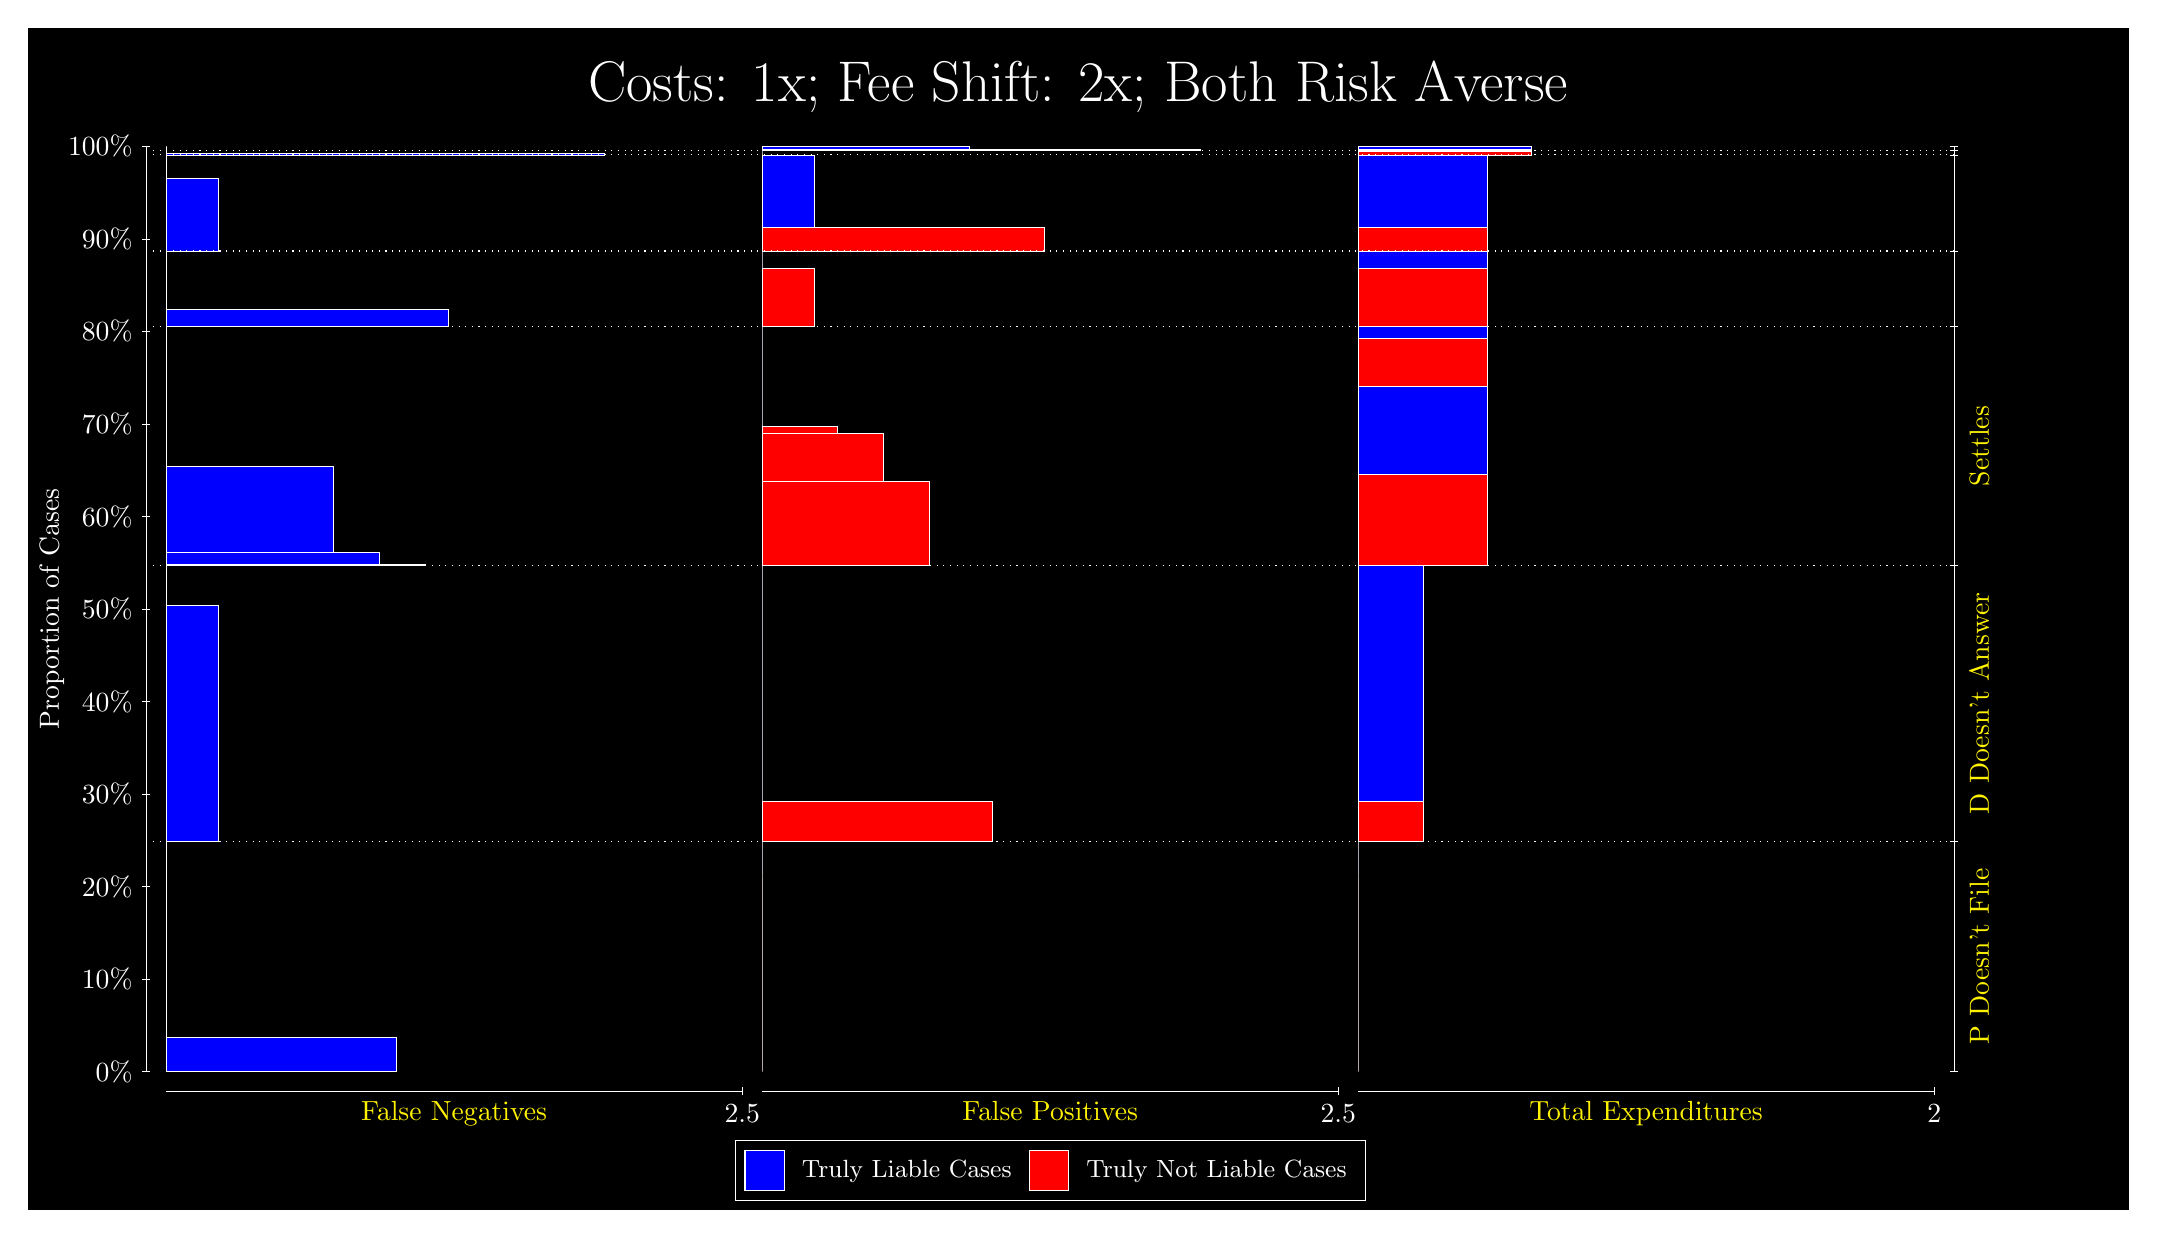
\begin{tikzpicture}
\draw[fill=black] (0,0) rectangle (26.667,15);
\draw[text=white] (0,13.5) rectangle (26.667,15) node[midway] {\huge Costs: 1x; Fee Shift: 2x; Both Risk Averse};
\draw[white, very thin] (1.5,1.75) -- (1.5,13.5);
\node[rotate=90, text=white, anchor=center] at (0.3, 7.625) {Proportion of Cases};
\draw[white, very thin] (1.45,1.75) -- (1.55,1.75);
\node[text=white, anchor=east] at (1.45, 1.75) {0\%};
\draw[white, very thin] (1.45,2.925) -- (1.55,2.925);
\node[text=white, anchor=east] at (1.45, 2.925) {10\%};
\draw[white, very thin] (1.45,4.1) -- (1.55,4.1);
\node[text=white, anchor=east] at (1.45, 4.1) {20\%};
\draw[white, very thin] (1.45,5.275) -- (1.55,5.275);
\node[text=white, anchor=east] at (1.45, 5.275) {30\%};
\draw[white, very thin] (1.45,6.45) -- (1.55,6.45);
\node[text=white, anchor=east] at (1.45, 6.45) {40\%};
\draw[white, very thin] (1.45,7.625) -- (1.55,7.625);
\node[text=white, anchor=east] at (1.45, 7.625) {50\%};
\draw[white, very thin] (1.45,8.8) -- (1.55,8.8);
\node[text=white, anchor=east] at (1.45, 8.8) {60\%};
\draw[white, very thin] (1.45,9.975) -- (1.55,9.975);
\node[text=white, anchor=east] at (1.45, 9.975) {70\%};
\draw[white, very thin] (1.45,11.15) -- (1.55,11.15);
\node[text=white, anchor=east] at (1.45, 11.15) {80\%};
\draw[white, very thin] (1.45,12.325) -- (1.55,12.325);
\node[text=white, anchor=east] at (1.45, 12.325) {90\%};
\draw[white, very thin] (1.45,13.5) -- (1.55,13.5);
\node[text=white, anchor=east] at (1.45, 13.5) {100\%};

\draw[white, very thin] (24.457,1.75) -- (24.457,13.5);
\draw[white, very thin] (24.407,1.75) -- (24.507,1.75);
\node[anchor=west] at (24.407, 1.75) {};
\draw[white, very thin] (24.407,4.6747) -- (24.507,4.6747);
\node[anchor=west] at (24.407, 4.6747) {};
\draw[white, very thin] (24.407,8.18) -- (24.507,8.18);
\node[anchor=west] at (24.407, 8.18) {};
\draw[white, very thin] (24.407,11.209) -- (24.507,11.209);
\node[anchor=west] at (24.407, 11.209) {};
\draw[white, very thin] (24.407,12.17) -- (24.507,12.17);
\node[anchor=west] at (24.407, 12.17) {};
\draw[white, very thin] (24.407,13.392) -- (24.507,13.392);
\node[anchor=west] at (24.407, 13.392) {};
\draw[white, very thin] (24.407,13.45) -- (24.507,13.45);
\node[anchor=west] at (24.407, 13.45) {};
\draw[white, very thin] (24.407,13.5) -- (24.507,13.5);
\node[anchor=west] at (24.407, 13.5) {};

\draw[white, very thin, fill=blue] (1.75,1.75) rectangle (4.6775,2.1847);
\draw[white, very thin, fill=red] (1.75,2.1847) rectangle (1.75,4.6747);
\draw[white, very thin, fill=blue] (1.75,4.6747) rectangle (2.4087,7.6705);
\draw[white, very thin, fill=red] (1.75,7.6705) rectangle (1.75,8.18);
\draw[white, very thin, fill=blue] (1.75,8.18) rectangle (5.0435,8.1933);
\draw[white, very thin, fill=blue] (1.75,8.1933) rectangle (4.458,8.3401);
\draw[white, very thin, fill=blue] (1.75,8.3401) rectangle (3.8725,9.4395);
\draw[white, very thin, fill=red] (1.75,9.4395) rectangle (1.75,11.209);
\draw[white, very thin, fill=blue] (1.75,11.209) rectangle (5.3362,11.425);
\draw[white, very thin, fill=red] (1.75,11.425) rectangle (1.75,12.17);
\draw[white, very thin, fill=blue] (1.75,12.17) rectangle (2.4087,13.088);
\draw[white, very thin, fill=red] (1.75,13.088) rectangle (1.75,13.392);
\draw[white, very thin, fill=blue] (1.75,13.392) rectangle (7.3123,13.41);
\draw[white, very thin, fill=red] (1.75,13.41) rectangle (1.75,13.45);
\draw[white, very thin, fill=red] (1.75,13.45) rectangle (1.75,13.468);
\draw[white, very thin, fill=blue] (1.75,13.468) rectangle (1.75,13.5);
\draw[white, very thin, fill=red] (9.3189,1.75) rectangle (9.3189,4.24);
\draw[white, very thin, fill=blue] (9.3189,4.24) rectangle (9.3189,4.6747);
\draw[white, very thin, fill=red] (9.3189,4.6747) rectangle (12.246,5.1842);
\draw[white, very thin, fill=blue] (9.3189,5.1842) rectangle (9.3189,8.18);
\draw[white, very thin, fill=red] (9.3189,8.18) rectangle (11.441,9.241);
\draw[white, very thin, fill=red] (9.3189,9.241) rectangle (10.856,9.8533);
\draw[white, very thin, fill=red] (9.3189,9.8533) rectangle (10.27,9.9492);
\draw[white, very thin, fill=blue] (9.3189,9.9492) rectangle (9.3189,11.209);
\draw[white, very thin, fill=red] (9.3189,11.209) rectangle (9.9776,11.953);
\draw[white, very thin, fill=blue] (9.3189,11.953) rectangle (9.3189,12.17);
\draw[white, very thin, fill=red] (9.3189,12.17) rectangle (12.905,12.474);
\draw[white, very thin, fill=blue] (9.3189,12.474) rectangle (9.9776,13.392);
\draw[white, very thin, fill=red] (9.3189,13.392) rectangle (9.3189,13.433);
\draw[white, very thin, fill=blue] (9.3189,13.433) rectangle (9.3189,13.45);
\draw[white, very thin, fill=red] (9.3189,13.45) rectangle (14.881,13.468);
\draw[white, very thin, fill=blue] (9.3189,13.468) rectangle (11.954,13.5);
\draw[white, very thin, fill=red] (16.888,1.75) rectangle (16.888,4.24);
\draw[white, very thin, fill=blue] (16.888,4.24) rectangle (16.888,4.6747);
\draw[white, very thin, fill=red] (16.888,4.6747) rectangle (17.711,5.1842);
\draw[white, very thin, fill=blue] (16.888,5.1842) rectangle (17.711,8.18);
\draw[white, very thin, fill=red] (16.888,8.18) rectangle (18.534,9.3369);
\draw[white, very thin, fill=blue] (16.888,9.3369) rectangle (18.534,10.45);
\draw[white, very thin, fill=red] (16.888,10.45) rectangle (18.534,11.062);
\draw[white, very thin, fill=blue] (16.888,11.062) rectangle (18.534,11.209);
\draw[white, very thin, fill=red] (16.888,11.209) rectangle (18.534,11.953);
\draw[white, very thin, fill=blue] (16.888,11.953) rectangle (18.534,12.17);
\draw[white, very thin, fill=red] (16.888,12.17) rectangle (18.534,12.474);
\draw[white, very thin, fill=blue] (16.888,12.474) rectangle (18.534,13.392);
\draw[white, very thin, fill=red] (16.888,13.392) rectangle (19.083,13.433);
\draw[white, very thin, fill=blue] (16.888,13.433) rectangle (19.083,13.45);
\draw[white, very thin, fill=red] (16.888,13.45) rectangle (19.083,13.468);
\draw[white, very thin, fill=blue] (16.888,13.468) rectangle (19.083,13.5);
\draw[white, dotted] (1.5,4.6747) -- (24.457,4.6747);
\draw[white, dotted] (1.5,8.18) -- (24.457,8.18);
\draw[white, dotted] (1.5,11.209) -- (24.457,11.209);
\draw[white, dotted] (1.5,12.17) -- (24.457,12.17);
\draw[white, dotted] (1.5,13.392) -- (24.457,13.392);
\draw[white, dotted] (1.5,13.45) -- (24.457,13.45);
\draw[white, very thin] (1.75,1.5) -- (9.0689,1.5);
\node[text=yellow, anchor=north] at (5.4094, 1.5) {False Negatives};
\draw[white, very thin] (9.0689,1.45) -- (9.0689,1.55);
\node[text=white, anchor=north] at (9.0689, 1.45) {2.5};

\draw[white, very thin] (9.3189,1.5) -- (16.638,1.5);
\node[text=yellow, anchor=north] at (12.978, 1.5) {False Positives};
\draw[white, very thin] (16.638,1.45) -- (16.638,1.55);
\node[text=white, anchor=north] at (16.638, 1.45) {2.5};

\draw[white, very thin] (16.888,1.5) -- (24.207,1.5);
\node[text=yellow, anchor=north] at (20.547, 1.5) {Total Expenditures};
\draw[white, very thin] (24.207,1.45) -- (24.207,1.55);
\node[text=white, anchor=north] at (24.207, 1.45) {2};

\node[text=yellow, centered, rotate=90] at (24.777, 3.2124) {P Doesn't File};
\node[text=yellow, centered, rotate=90] at (24.777, 6.4273) {D Doesn't Answer};
\node[text=yellow, centered, rotate=90] at (24.777, 9.6943) {Settles};





\draw (12.978300999999998,1.5) node[draw=none] (baseCoordinate) {};
\begin{scope}[align=center]
        \matrix[scale=0.5, draw=white, below=0.5cm of baseCoordinate, nodes={draw}, column sep=0.1cm]{
            \node[rectangle, draw, minimum width=0.5cm, minimum height=0.5cm, fill=blue] {}; &
            \node[draw=none, font=\small, text=white] (B) {Truly Liable Cases}; &
            \node[rectangle, draw, minimum width=0.5cm, minimum height=0.5cm, fill=red] {}; &
            \node[draw=none, font=\small, text=white] (B) {Truly Not Liable Cases}; \\
            };
\end{scope}

\end{tikzpicture}
\end{document}